\documentclass{mpaper}

\begin{document}

\title{TactiHelm: A Vibrotactile Helmet for Cycling Safety}
\author{Lewis Trundle}
\matricnum{2469635t}

\maketitle

\begin{abstract}
According to Simon Peyton Jones, an abstract should address
four key questions. First, what is the problem that this
paper tackles? Second, why is this an interesting problem?
Third, what is the solution this paper proposes?
Finally, why is the proposed solution a good one?
\end{abstract}

\section{Introduction}

\subsection{Motivation}
Each year, road-traffic accidents account for 1.35 million deaths worldwide, with cyclists comprising 41,000 of these fatalities \cite{world2018global}. The economic burden associated with road accidents in the EU alone is estimated to amount to 236 billion euros annually \cite{costoftransport}. Despite the EU achieving an average annual reduction of 3\% in motor vehicle related fatalities, between 2010 and 2018, the fatality rate for cyclists remained the same across that period \cite{adminaite2020safe} - emphasising the lack of attention towards cyclists regarding road safety.

One of the primary causes of cyclist fatalities is collisions with motorised vehicles \cite{BIL20101632}, with 78\% of cyclist fatalities in the EU due to bicycle-to-vehicle collisions \cite{adminaite2015making}. Although a collision with another vehicle may occur from any angle, situations where the offending vehicle crashes into the cyclist from behind cause the largest proportion of fatalities of all crash directions \cite{BIL20101632}. Despite a large body of research investigating how cyclist safety can be improved using safety systems implemented within other road vehicles \cite{scholliers2014potential, SILLA2017134, cieslik2019improving, 7929602, 10.1145/3434770.3459732}, few studies have explored how cyclist safety can be improved from the perspective of the cyclist \cite{10.1145/3490099.3511127, STROHAEKER2022151}. 

Studies investigating the cognitive demand of cycling has shown that novice cyclists often struggle to accomplish cognitive tasks which are necessary for traffic safety, such as looking for traffic and identifying the type of intersection \cite{https://doi.org/10.1002/acp.2350050205}. To aid cyclists, safety technology such as rear-view bike radars \cite{garminradar} help reduce cognitive load, by delivering warning messages about approaching vehicles both visually and audibly. An obvious benefit of auditory messages is that they do not consume the visual sensory channel. However, auditory messages have been shown to be difficult to understand in noisy environments \cite{noisyenv} and in situations such as when the cyclist is listening to music, something which many admit to doing \cite{DEWAARD2011626}.

A possible alternative message modality is vibrotactile. Previous work from Vo et al. \cite{10.1145/3411763.3451580} explored how this modality can be used for the purpose of cyclist safety, something which no other studies have done as of yet. Regarding where to encode vibrotactile stimulation, there are many options. Previous work have used belts \cite{10.1145/1613858.1613911, 10.1145/2449396.2449450, 10.1145/1060581.1060585}, vests \cite{729547, 998954, van2000tactile, 10.1145/2556288.2557404}, and even bicycles \cite{10.1145/2371574.2371631, 10.1145/3290605.3300850}, as mediums for vibrational stimuli, with products such as attachable handlebar grips which can provide vibrotactile feedback \cite{smartgrips}. However, an unexplored area is the potential of the helmet. Few studies have explored how vibrotactile stimuli can be used in helmets \cite{10.1007/978-3-642-39802-5_3, yamauchi2020vibro} and even fewer have investigated how this can be applied in the context of cycling \cite{krauss2021head}.
 

\subsection{Problem Statement and Aim}
We aim to develop a vibrotactile helmet which can improve cycling safety - helping to lower the number of cyclist fatalities. More specifically, we aim to develop a hazard notification system using vibration for cyclists, able to effectively communicate to the cyclist when a vehicle from behind is approaching. 

The system is restricted to the context of notifying of vehicles behind the user, as from our motivation, we identify this as a dangerous situation, with little existing work to aid cyclists in this context. By focusing our system to work in this specific context, we aim to make the most impact in terms of improving cyclist safety.

Regarding developing this system, we first investigate the best metric (or metrics) to convey to a cyclist, to appropriately inform them of approaching vehicles. We hypothesise that this would simply be \textit{distance}. However, categories of such a metric can be arbitrary - what specific distances do terms such as \textit{far} or \textit{near} mean to a cyclist? We hope to distinguish such meanings in this project.

Secondly, we explore how this information can be encoded using vibrotactile cues. This modality is chosen due to its potential to provide feedback with minimal distraction. Therefore, our chosen coding method should be able to accurately represent the appropriate metric, with minimal diversion of the cyclists' attention. Furthermore, we investigate how this system can be incorporated into a helmet - our chosen medium due to the unexplored potential of bicycle helmets for interaction. We seek to answer which region of the head is best to place vibrotactile motors, and what parameters of the vibrations are most suitable to encode our vibrotactile cues.

Finally, we will evaluate the system in a real-world user study, to learn cyclists' thoughts regarding its usefulness for cycling in real-life. By testing the system in realistic conditions, we hope to discover if it achieves its purpose of improving cycling safety.

\section{Background}

here is little literature on the use of vibrotactile feedback while cycling, and of the existing corpus, few relate to the problem of cyclist safety. To address this issue, we survey four broad areas of research, and combine the insights we gather to inform our approach to developing TactiHelm. We first examine existing literature regarding \textit{in-vehicle} hazard notification systems for cyclists. We then explore how different feedback modalities have been used in cycling. Finally, we review the ways in which vibrotactile stimuli can be used to encode information, and how this can be applied to the head.

\subsection{Hazard Notification for Cyclist Safety}
The idea of a hazard notification system was first explored in 1992 by Horowitz and Dingus \cite{doi:10.1177/154193129203601320}. They proposed various design approaches, such as adjusting the warning intensity based off the detected collision time, and employing different signal modalities to convey various warning severities - concepts which have been often used in later research. However, it was not until 1996 where one of the earliest hazard detection systems emerged \cite{566402}. While not explicitly labelled as a hazard detection system, this project combined radar and vision technologies to create a system which could detect and classify road vehicles ahead of the car, then appropriately change lanes to avoid collision. This idea of detecting vehicles in-front was continued in subsequent research by Huang et al. who developed a warning system which could detect lane boundaries and successfully detect a vehicle in-front with 97\% accuracy \cite{1307429}.

These early in-vehicle warning systems are all examples of Intelligent Transport Systems (ITSs) - a series of information and communications technologies which aim to improve the safety of transportation \cite{its}. Despite research into various types of ITSs, few address how the safety of vulnerable road users (VRUs), such as cyclists, can be improved \cite{Scholliers2017}. Silla et al. \cite{SILLA2017134} performed a quantitative safety impact assessment of five different types of ITSs, to evaluate which has the greatest potential to improve cyclist safety. They found that by 2030, the Pedestrian and Cyclist Detection System + Emergency Braking (an in-vehicle system which uses detection sensors to detect pedestrians/cyclists in front of a forward moving vehicle to warn and automatically brake) would have the greatest effect. The PROSPECT project \cite{cieslik2019improving}, funded by the European Commission, further improves the effectiveness of detection systems. Not only is it able to detect VRUs, but it can also detect their intentions - allowing the vehicle to take pre-emptive measures, such as changing its speed or course, to avoid a collision. This project is estimated to reduce the number of seriously injured people in the EU by anywhere up to 2,500 people by 2030.

Another promising ITS mentioned by Silla et al. \cite{SILLA2017134} is Bicycle to Vehicle communication (B2V) systems. Jenkins et al. created a system which could bring cyclists onto the US Connected Vehicles Program \cite{usdot} - an initiative designed to bring vehicles onto a Vehicle-to-Everything (V2X) network\footnote{The \textit{'Everything'} part of V2X refers to any entity which has an impact or can be impacted by a vehicle. Typically, V2X is a combination of Vehicle-to-Vehicle (V2V) and Vehicle-to-Infrastructure (V2I) networks. In this specific case, Jenkins et al. aims to also include a Vehicle-to-Cyclist (V2C) network.}. This was done by outfitting cyclists with a low-cost DSRC-WAVE\footnote{Dedicated Short-Range Communications for Wireless Access in Vehicular Environments (DSRC-WAVE) is currently one of the only ways to provide V2X networks, with high reliability and low latency.} solution which allowed them to receive basic safety messages. From this, they created a multimodal hazard notification system which would deliver these safety messages using audio and haptic cues. By varying signal parameters, they were able to create a unique vocabulary of cues which cyclists could learn. This was delivered via a standard smartphone speaker and Boreal Bikes’ smrtGRiPs \cite{smartgrips}. Although the paper does not describe exactly how these cues were encoded, it does describe the five hazard categories used to decide which action to recommend to the cyclist - ranging from cautionary messages to suggesting immediate action.

Lujic et al. combines the idea of cyclist detection systems and connected networks, to create InTraSafEd5G \cite{10.1145/3434770.3459732}, a system which can predict when pedestrians and cyclists will enter a vehicles' blind spot at intersections. By installing nodes across various traffic lights around Vienna, the authors create an Edge network which is able to detect critical situations and deliver early warning messages to drivers in real-time using 5G. These warnings are delivered both visually and audibly to a driver’s mobile phone. This work highlights the potential of combining various types of ITSs to create a system which enhances cyclist safety. However, the described system only provides a single type of notification to the driver, only alerting them of whether a potential collision is possible. An improved system may deliver different types of notifications which is able to effectively communicate more information about the potential collision.

Despite the potential for improving cyclist safety using ITSs, pre-existing attitudes and perceptions affect the acceptance of such systems. Angelis et al. \cite{de2017negative} investigated how attitudes towards cyclists effect how likely a driver is to use an in-vehicle cyclist detection system. They found that drivers who already express a negative representation of cyclists are more unlikely to use a new technology, compared to those who do not. This is further explored by Berge et al. \cite{berge2022cyclists} who studied acceptance from the perspective of the cyclist, exploring their beliefs and attitudes towards being equipped with human-machine interfaces (HMIs) for communication with smart-traffic. Through analysis of questionnaire responses and interviews, the authors identified that cyclists were worried about using HMIs as the responsibility of safety would be imposed on themselves, regardless of whether a situation warrants they take immediate action. 


\subsection{Feedback Modalities in Cycling}
Wolfe et al. \cite{wolfe2016distracted} investigated the different types of distractions which cyclists commonly face, finding that auditory distractions were most common, followed shortly by visual ones. Despite little research into \textit{‘distracted biking’} \cite{mwakalonge2014distracted} it is generally believed that cyclists’ use of mobile phones is at the root of the cause. Angelis et al. \cite{doi:10.1080/19439962.2019.1591559} studied the relationship between smartphone usage while cycling and frequency of crashes, finding that the usage of a smartphone led to an increased crash risk. With over half a surveyed population admitting to using their mobile device on every trip \cite{GOLDENBELD20121} and 17\% of the population admitting to using one during every ride \cite{goldenbeld2010use}, there have been calls to put legislation in place to prevent the use of smartphones while cycling \cite{banphoneuse}. However, Angelis et al.'s study found that the link between smartphone usage and increased crash risk was not true for their female subsample, and only applied to their male subset. Although they recommend investigating this further, this finding is also backed by other studies exploring differences in cycling behaviours based on factors such as gender \cite{BEHNOOD201735}. Furthermore, the authors admit to limitations in their study, such as the unreliability of participants remembering crashes. While some studies have investigated ways to improve smartphone interaction while cycling to reduce distraction \cite{10.1145/3544548.3580971, 10.1145/3152832.3152871} other approaches have investigated alternative interaction modalities, which don’t make use of the visual sensory channel.

The concept of utilising different sensory channels to convey information is an idea studied by Wickens \cite{wickens1984processing} and Wickens and Liu \cite{doi:10.1177/001872088803000505}, who explored ‘Multiple Resource Theory’ - a model of human information processing which predicts that attention is a limited cognitive resource that can be allocated across different tasks and modalities. The model implies that multiple sensory channels can be used simultaneously (within the cognitive load of the individual), without any individual one degrading the processing performance of the human operator. Seeking to take advantage of this concept, Wickens suggests that tasks can be configured to utilise multiple sensory channels - exploiting our information-processing capabilities.

In the context of cycling, multiple works would explore the potential of utilising such a model, by developing tactile displays to aid navigation. One of the earliest instances of this was by Pielot et al. \cite{10.1145/2371574.2371631} who developed Tacticycle - a bicycle with a minimal set of navigational cues encoded into the handlebars, to guide tourists to points of interests. Direction was encoded via the relative intensity across both handlebars. For example, a 45\degree{} angle to the right was indicated by 25\% intensity vibration in the left handlebar and a 75\% intensity vibration in the right. This coding method proved effective, as participants in a study were able to understand the tactile cues and none of them reported losing orientation. However, the authors acknowledge that their testing environment was geographically constraint, and that it was likely participants could find the correct way to their destination as long as they travelled roughly in the right direction. Steltenpohl and Bouwer \cite{10.1145/2449396.2449450} created Vibrobelt - a vibrotactile belt also developed to aid navigation while cycling . By analysing the visual focus and spatial knowledge acquisition of participants, the authors found that the use of Vibrobelt increased participants ability to recall images from the route, but were generally slower at navigating and recalling the route - showing a lesser contextual understanding. Peeters et al. \cite{peeters2019vibrotactile} investigated response times of vibrotactile cues during various levels of physical cycling exercise. By attaching vibrotactile motors to participants' spine and thighs, they showed that vibrotactile signals were perceivable in both a stationary position, and during diverse levels of physical effort. Furthermore, they showed that cyclists' reaction time to stimuli shortened as they were cycling with greater effort. However, the study does not investigate the tactile perception of other body parts while cycling, such as the head.

Strohaeker et al. \cite{STROHAEKER2022151} investigated the effect of unimodal warnings on cyclists to prevent collisions, specifically comparing acoustic and vibrotactile warnings. The results found that warnings, especially acoustic, were effective at shortening response times to potential collisions. Though, vibrotactile warnings could also be effective for a system which does not require urgent reactions from the cyclist. This study however, did not consider how multimodal warnings could be used. The effects of unimodal and multimodal cues would be investigated by Matviienko et al. \cite{10.1145/3290605.3300850, 10.1145/3229434.3229479} who compared the effectiveness of delivering navigational instructions to child cyclists using visual, auditory, and vibrotactile feedback. Visual and auditory cues were delivered using flashing lights and speakers inside a bicycle helmet, and vibrotactile cues were delivered using the bicycles' handlebars - similar to Tacticycle \cite{10.1145/2371574.2371631}. Results from their study showed that unimodal cues were easier to recognise, and so were best used to indicate directions, but multimodal cues were best used to communicate when immediate action is required as it demonstrated shorter reaction times and better understandability. However, due to the sample size and age of the participants, the authors acknowledge that these findings may not be generalisable to the public. These findings are backed by Sawitzky et al. \cite{10.1145/3490099.3511127, mti6010003} who compared different awareness message modalities for cyclists to avoid dooring - a type of collision where a parked vehicle door suddenly opens onto the path of an incoming cyclist. The authors compared the effectiveness of using combinations of visual messages, auditory icons, and voice messages for delivering warning notifications. The results showed that participants generally preferred the multimodal combination of visual messages and auditory icons. Although the study does not provide any evidence for how tactile feedback could be used, it does suggest it be studied for future work.

Despite the potential of using different communication modalities while cycling, there are drawbacks to each. Waard et al. \cite{DEWAARD2011626} discovered that 68\% of auditory cues were missed when participants were listing to music. Notably, no negative effects towards participants auditory perception were recorded when they only used one earbud. Although Wolfe et al. \cite{wolfe2016distracted} suggests these effects can be reduced using bone conducing headphones\footnote{These differ from regular headphones in that, instead of projecting air pressure waves directly into a wearers' ear, they instead use the cheekbones to transfer auditory signals directly to the cochlea \cite{littler1952hearing}.}, May and Walker \cite{may2017effects} found that when distractor sounds were played through them, a wearers' ability to localise critical environment sounds worsened. Erdei et al. \cite{erdei2020comparing, doi:10.1080/15389588.2021.1985113} reported that the perception of vibrotactile signals during cycling worsen in environments where the surface causes haptic interference. However, they suggested this could be overcome by adjusting how the vibrotactile stimuli was delivered to the cyclist. An effective way of delivering stimuli was shown by Tacticyle \cite{10.1145/2371574.2371631}, where they delivered vibrations through the handlebars as they believed, \textit{“these are the only parts of the bicycle that the rider constantly touches during the ride”}. This statement would be proven correct by Hochleitner et al. \cite{10.1145/3152832.3152871} who found that cyclists like to keep their hands on the handlebars as much as possible. Furthermore, Porcheron et al. \cite{10.1145/3544548.3580971} further studied cyclists use of technology while cycling and through findings of an ethnographic study, they introduced the concept that the handlebars are a ‘zonal space’. This alluded to the possibility of expanding the potential stimuli vocabulary, by encoding information across various zones of the handlebars. Companies have even capitalised on the capabilities of the handlebars for vibrotactile feedback, with products such as smrtGRiPs \cite{smartgrips} which can be attached to the handlebars of any bicycle.


\subsection{Coding Information Using vibrotactile Stimuli}
\subsubsection{Coding Direction Using Veridical and Illusionary Stimuli}
Much early work utilising vibrotactile stimuli would explore how tactile displays could be incorporated alongside visual displays, to extend a computer systems’ functionality. Tan and Pentland \cite{629923}, investigated how tactile displays could be used in wearable computing - suggesting they could be used as directional displays to aid navigation. Ertan et al. \cite{729547} would shortly realise this idea of a wearable navigational display less than a year later in 1998, where they developed an adjustable vest which provides directional navigational instructions via vibrations. These directions were conveyed by vibrating a grid of motors - which were sewn into the back of the vest - in a specific pattern. For example, to indicate a right turn, the motors were activated sequentially, from left to right. Research into the design of such a haptic vest would continue over the years, including a study, investigating its efficiency in conveying directional instructions across different gravity conditions \cite{998954}. Although the study found that the perceived intensity of vibrotactile signals did not change across the varying conditions, it did comment on the effect that cognitive load has on a persons ability to interpret tactile signals - suggesting the need for further psychophysical experiments investigating haptic perception.

This method of communicating direction makes use of a vibrotactile illusion known as ‘sensory saltation' - a phenomenon in which successive pulses delivered to equidistant regions of a body part simulate the feeling of movement across the stimulus area \cite{geldard1975sensory}. Lederman and Jones \cite{5710913} and Lee et al. \cite{s150407913} studied different types of sensory illusions, dividing haptic illusions into two types: saltation, and funneling - the illusion of perceiving a single sensation at the centre of two or more simultaneously presented stimuli which are close in proximity. The use of such illusions has the potential to reduce the number of required actuators \cite{10.1007/s00779-015-0894-4}, and earlier studies showed that these illusions are highly robust. Gardner and Spencer \cite{gardner1972sensory} studied funneling, by placing three stimulators spaced 30mm apart on participants forearms and simultaneously activating them. In 80\% of the trials, participants reported feeling a stimulation within a 20mm band of the middle stimulator. Cholewiak and Collins \cite{cholewiak2000generation} compared the perception of veridical and saltatory sensations. When presenting participants with both types of sensations, the majority of responses reported feeling the same sensation - highlighting the effectiveness of using saltation to mimic veridical signals. However, a study by Peeters et al. \cite{peeters2019vibrotactile} contradict these findings. By measuring the perception of vibrotactile signals at the thigh and spine, they showed that illusionary signals were less perceptible than veridical signals, with participants often feeling the individual veridical stimuli during the illusion conditions.

Later studies would often utilise veridical signals for coding direction, such as one conducted by van Erp \cite{van2000tactile}, which used the on-body location of the veridical vibration to indicate the direction of travel. Using a haptic vest similar to Ertan et al. \cite{729547}, they instead attached motors around the axial (horizontal) plane of the wearers body, allowing directions in a 360\degree{} circumference to be conveyed. The use of such a coding scheme has the benefit of only requiring a linear array of motors, and would lead to such tactile displays being implemented on smaller wearables, such as belts \cite{10.1145/1613858.1613911, 10.1145/2449396.2449450, 10.1145/1060581.1060585}. Only a small number of studies have investigated how funneling can be use, such as one conducted by Kim et al. \cite{10.1007/s00779-015-0894-4}, who demonstrated how funneling and saltation could be extended to 2D objects to create an \textit{"out of the body"} sensation. They attached vibrators to the rear of a mobile device and a phantom sensation was created in the middle area of the phone by varying the relative intensities of vibrations (in the case of funneling) and varying the inter-stimulus intervals (in the case of saltation). Participants were able to feel a phantom sensation in the gap between their two hands holding the mobile device - demonstrating how a greater number of stimulus loci can be created using only a small number of actuators.


\subsubsection{Coding Distance Using Multiple Parameters}\label{sec:coding-distance}
Although a simple navigational system may only convey direction to a user, a more effective one would also typically convey an idea of distance \cite{burntt2002empirical}. Parameters to encode information is studied by van Erp, who explores spatial and temporal effects of vibrotactile stimuli \cite{guidelines}. The paper serves as a set guidelines for implementing a vibrotactile system and suggests that a vibrotactile display affords four parameters which can be adjusted: the location, timing, frequency, and amplitude of a vibration. How parameters such as these can be used is described by Brewster and Brown \cite{10.5555/976310.976313}, who introduce \textit{Tactons} - structured, abstract messages, whose meaning is encoded using the parameters of cutaneous perception\footnote{Cutaneous perception refers to receptors under the surface of the skin. The cutaneous senses are multimodal and includes sensations of temperature, pressure, and vibration.}. The authors expand on the parameters suggested by van Erp, explicitly describing how temporal characteristics of a vibration, such as rhythm and duration can be used.

Previous studies have investigated how these parameters can be used to create coding schemes for distance. van Erp et al. \cite{10.1145/1060581.1060585} investigated the effectiveness of different distance coding schemes to aid navigation for pedestrian participants. Two main categories of distance coding schemes were used; the first was a monotonic relation between distance and rhythm - as the distance got smaller, the rhythm got faster. The second category was a three-phase model, which varied the delay duration between vibration pulses, depending on which phase of the navigation task the participant was in. Navigational directions were encoded by the location of the vibrotactile motors on a belt which participants wore. Notably, there was no difference found in participant performance when comparing those with access to distance information, to those without - concluding that this may be due to the confounding of the distance information with the temporal resolution of the direction information. Straub et al. \cite{5326374} conducted a similar experiment, also using a vibrotactile belt to perform navigational tasks with pedestrians. Three experiments were preformed to explore how the encoding of distance using the parameters of rhythm, intensity, and frequency, affected the walking speed of participants. Similarly to van Erp et al. \cite{10.1145/1060581.1060585}, no notable differences to walking speed were found. However, this is likely attributable to the confounding of parameters, as both rhythm and intensity are simultaneously varied in the experimental coding schemes.

The inconclusive findings from van Erp et al. \cite{10.1145/1060581.1060585} and Straub et al. \cite{5326374} identified a need to further explore how distance can be coded using temporal aspects of vibrotactile stimulation, something which the skin is sensitive to \cite{doi:10.1068/p5014}. McDaniel et al. \cite{10.1145/1520340.1520718} utilised tactile rhythms to create a coding scheme to convey intimate, personal, interpersonal, and social distances to the blind. The duration of a pulse was kept to a constant 50ms, but as the distance increased, the delay between pulses increased, similar to van Erp et al.'s monotonic scheme \cite{10.1145/1060581.1060585}. However, this experiment proved effective, and showed that given a small training period, users were able to effectively identify different tactile rhythms and associate them with their respective distances. Pielot et al. \cite{10.1145/1753326.1753581} further studied distance encodings by developing a tactile display which presents the position and distance of other team members in a fast-paced 3D multiplayer game. They compared rhythm-based, duration-based, and intensity-based schemes. Participants found their rhythm-based scheme the easiest to judge distance. Furthermore, they proved it was possible to accurately use vibrotactile signals to convey distance in an environment with high cognitive demand. Asif et al. \cite{10.1145/1868914.1868923} further studied these parameters, but instead explored how they could be combined to compare three rhythm-based schemes: rhythm only, rhythm and intensity, and rhythm and duration. These schemes were used in-vehicle, to indicate different categories of distance until an approaching turn. The results found that the combination of rhythm and duration (where the pulse duration stayed the same but the number of pulses decreased as the distance decreased) was the easiest for participants to learn and led to the smallest amount of navigational mistakes. This finding motivated Prasad et al. \cite{10.1145/2556288.2557404} to develop HaptiMoto - a wearable vest which provides vibrotactile feedback regarding upcoming turns for motorcyclists. Through a user study, they were able to prove that the rhythm and duration coding scheme for distance, as found by Asif et al. \cite{10.1145/1868914.1868923}, was effective at providing navigational instructions to motorcyclists. However, the authors note that this was only studied at low speeds of below 25 mph.


\subsection{Vibrotactile Stimulation on the Head}
\subsubsection{Spatial Acuity and the Midline Effect}
An early investigation into the spatial acuity of the head was performed by Gilliland and Schlegel \cite{doi:10.1177/001872089403600410} who studied localisation ability for various configurations of 4 to 12 tactors placed across the coronal plane of the head. Specifically, tactors were placed across the parietal meridian (from ear to ear). They found that optimal tactile detection and localization accuracy occurred when using six tactors - with a 93\% accuracy. More than this, and both the accuracy and reaction time worsened. Myles and Kalb \cite{headguidelines} also assessed tactile perception - comparing different regions of the head, using various configurations of eight tactors. They found that the scalp (namely the parietal, central and frontal regions) were the least sensitive loci on the head, whereas, the regions around the axial plane of the head (namely the forehead, occipital, and temple regions) were the most sensitive loci. These different regions can be seen in Figure \ref{fig:head-regions}. Myles et al. \cite{MYLES2015177} continued studying how the effects of vibrotactile stimulation varied across regions of the head, by investigating to what effect hair density has on vibration sensitivity. Although known to cause lessened vibrotactile sensitivity, they found that the density of hair on the skin only has a small effect. More so, this effect is confined to only the regions of the head which are the least sensitive.

de Jesus Oliveira et al. \cite{7463147} studied the spatial resolution of the head, specifically, comparing the more sensitive regions as identified by Myles and Kalb \cite{headguidelines}. Namely, the forehead (referred to as frontal in this paper), temporal, occipital, and frontotemporal regions. Although they found that the forehead was the most accurate region for spatial discrimination of vibrotactile stimuli, their results also showed that the centre of the occipital region had high precision. Furthermore, they found that as the distance from the head midline increased, the precision for spatial discrimination decreased - naming this phenomenon as the \textit{Midline Effect}. Although this was the first direct reporting of this effect, it had been indirectly reported on earlier by van Erp \cite{1406917} who studied how spatio-temporal characteristics of vibrotactile patterns on the torso effects spatial acuity. He hypothesised multiple reasons for this phenomenon, such as suggesting the body midline is like an anchor point - allowing aid in absolute localization, or that the central nervous system has specific characteristics for processing stimuli. Regardless of the reason, de Jesus Oliveira et al. suggests further research is needed investigating the effect.


\subsubsection{Tactile Systems for the Head}
An early study investigating the role that vibrotactile stimulation can have in a helmet was conducted by Bertram et al. through The Tactile Helmet Project \cite{10.1007/978-3-642-39802-5_3}. Vibration actuators were placed around the headband of a helmet, to warn the wearer of imminent collisions and communicate the distance of detected objects. The device is designed with the philosophy of \textit{"active sensing”}, where the behaviour of the device changes depending on the context of use. This is accomplished by varying the type and intensity of a vibration by using a context-sensitive algorithm, which takes into account the walking speed of the wearer.

Yamauchi and Suzuki \cite{yamauchi2020vibro} demonstrated how a vibrotactile helmet could be used for hazard notification, specifically, in the context of motorcycling. The location of the vibration on the different regions of the head (the forehead, temporal, and occipital regions) corresponded to the direction of the hazard, whereas the strength of the vibration corresponded to the level of risk. They showed that the use of four directions and three levels of intensity was effective at notifying a wearer of an approaching hazard, even in winds of up to 100km/h.

However, in the context of cycling, the only study to the best of our knowledge which investigates how vibrotactile stimulation around the head can be used, was conducted by Krau{\ss} et al. \cite{krauss2021head}. This study developed a navigational headband which vibrated on the wearers head in the direction of travel - using 12 actuators for a spatial resolution of 30\degree{}. They demonstrated that vibrotactile stimulation could be used on the head whilst cycling, without the wearer reporting discomfort or distraction. Although the use of a headband is similar to a helmet, we recognise that no studies have explored how vibrotactile stimulation can be delivered via a helmet to aid cycling.


\section{The TactiHelm System}

The following section details each part of the project, describing which stages have been completed, and which stages we are yet to complete. More specifically, it outlines the current implementation of the TactiHelm system, before describing the results from an initial user survey. Finally, it thoroughly describes the plan for two future studies. It is important to note that some details may change in future development of the project.
\subsection{TactiHelm System Design}\label{sec:system-design}
\subsubsection{Circuit Hardware}\label{sec:circuit-design}
The current TactiHelm helmet builds off previous work from Vo et al. \cite{10.1145/3411763.3451580}. The inside lining of the helmet is equipped with 10mm diameter, three volt ERM coin cell tactile actuators (tactors). The exact location, number, and spacing of these tactors is discussed in Section \ref{sec:helmet-design}. These actuators are driven by PWM signals from 0 to 3V generated by an Arduino Uno micro-controller \cite{arduinouno}, which is powered using a standard 9V battery. PWM can represent the use of an analogue signal \cite{kart2001pulse}, allowing us to more precisely vary the range of discrete values used to control the intensity of the tactile actuators. The Arduino Uno has six PWM pins, thus if we wish to vary the intensity of the actuators, we are limited to just six of them. The circuit is also equipped with an HC-06 Bluetooth Module, to allow for remote control over the actuators. This Bluetooth module communicates using Bluetooth Classic \cite{hc06}. A diagram of the full circuit can be seen in Figure \ref{fig:circuit}.

\begin{figure}[ht]
    \centering
    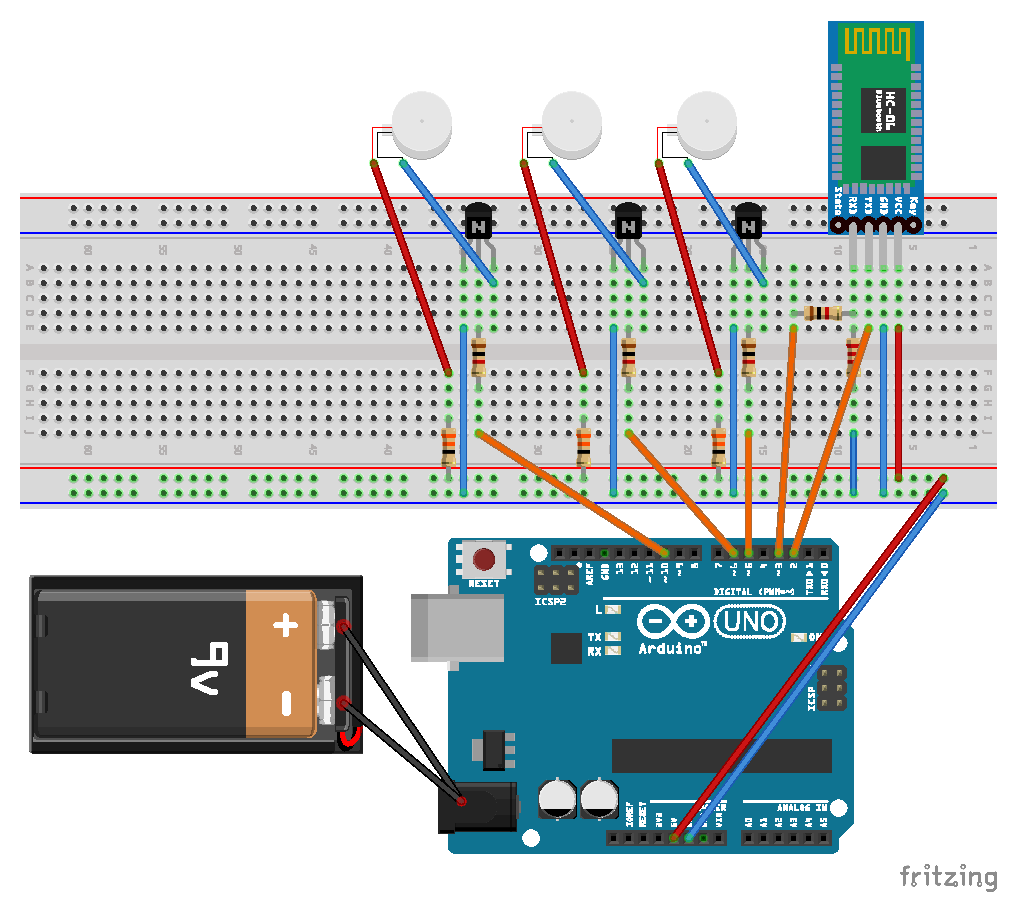
\includegraphics[width=0.75\textwidth]{images/circuit-design_bb.pdf}
    \caption{Figure shows the constructed circuit for TactiHelm. A voltage divider is used to limit the voltage level between the HC-06 Bluetooth Module and the Arduino \cite{bluetoothmodule}. The vibration motors require more power than the Arduino pins can provide, so NPN transistors are used to amplify the signal \cite{vibrationmotor}.}
    \label{fig:circuit}
\end{figure}


\subsubsection{Bike Radar Design}
On the other side of the TactiHelm system is the Garmin Varia RTL515 bike radar \cite{garminradar}. Designed to attach to the back of a bicycle, the radar can detect vehicles up to a range of 140 metres, with a viewing angle of 220\degree{}. The radar allows for two communication methods: Bluetooth Low Energy (BLE) and ANT+. Communicating using BLE provides us with access to the distance and speed of each detected vehicle. Notably, BLE does have limitations such as a smaller bandwidth compared to ANT+ \cite{bluetoothlimitations}. However, this is not a concern since only a small amount of data is being transferred. From this, the following questions remain:
\begin{itemize}
    \item Which metric (or metrics), from distance, speed, or some arbitrary combination of the two, is most suitable for signifying an approaching vehicle to a user?
    \item How can this metric be conveyed to a user? Should continuous values be encoded, or should the metric be defined into categories? What do these arbitrary categories mean to users? 
    \item How can this information be encoded using vibrotactile cues?
\end{itemize}

To answer the first question, a potential metric for our system is the \textit{following distance} of the car behind. Typically measured in seconds, the UK Government suggests that vehicles maintain at least a two-second gap from the vehicle in-front \cite{followdistance}. We can quite simply calculate the following distance using the distance and speed given to us by the bike radar. Answers to the other questions are explored with a lab-study investigating different cues and encodings, described in Section \ref{sec:lab-study}.


\subsubsection{App Design}
To allow communication between the bike radar and Arduino, a custom-built React Native application was developed, to act as an intermediary between the two devices, as seen in Figure \ref{fig:overall-system}. The current state of the application can run on an Android mobile phone; however, future versions of the app would ideally also run on an iOS device. Currently, the following functionality is possible with the application:
\begin{itemize}
    \item Connect to the HC-06 Bluetooth module using Bluetooth Classic
    \item Connect to the Garmin Varia using Bluetooth Low Energy
    \item Receive the distance and speed information of each detected vehicle from the bike radar.
    \item Manually turn on/off and control the vibration intensity of each connected actuator.
\end{itemize}

What remains to be implemented is a pipeline between the bike radar and Arduino. More specifically, the information received via BLE from the bike radar should be parsed and encoded into the relevant vibrotactile cues. However, this is not possible, until such encodings to cues are defined, as discussed further.

\begin{figure}[ht]
    \centering
    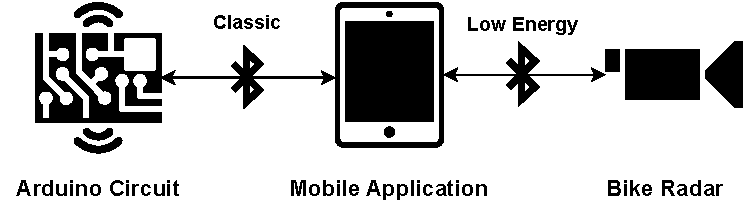
\includegraphics[width=0.75\textwidth]{images/overall-system.pdf}
    \caption{Figure shows the overall system design. The bike radar communicates to the mobile application using Bluetooth Low Energy, which in turn communicates to the Arduino circuit using Bluetooth Classic.}
    \label{fig:overall-system}
\end{figure}


\subsubsection{Coding Distance Using Rhythm and Location}
As previously mentioned in Section \ref{sec:coding-distance}, a vibrotactile display affords four parameters which can be adjusted: the location, timing, frequency, and amplitude of a vibration \cite{guidelines}. In our described system, the \textit{'intensity'} of a vibration is controlled by varying the voltage to the motor using pulse-width-modulation (as described in Section \ref{sec:circuit-design}). These changes in voltage results in simultaneous changes in frequency and amplitude, meaning the parameter \textit{'intensity'} is treated as a combination of these two parameters. However, whether these are suitable parameters for our system depends on how many intervals we wish to categorise distance, as frequency and amplitude only have 5-7 perceptually distinguishable levels \cite{guidelines}. From this, and for the sake of simplicity, we choose not to study how the intensity can be varied. Furthermore, it is known that the perception of a stimulus is effected by the waveform \cite{guidelines}. However, the vibration motors which we are using are only capable of producing sine waves, meaning we are limited to this waveform.

This leaves the parameters of location and timing to be used to encode distance. Many studies have investigated how timing (or more specifically, rhythm) can be used to represent different distances \cite{10.1145/1060581.1060585, 5326374, 10.1145/1520340.1520718, 10.1145/1753326.1753581, 10.1145/1868914.1868923}. In these studies, the distance is measured from a moving wearer, to a stationary point of interest (POI), where the wearer is moving towards the POI. However, in the context of our described system, the POI (the approaching vehicle) is moving towards the wearer, who is also travelling in the same direction. This motivates the need to study whether typical rhythm coding schemes for distance are still appropriate for use in our described context. Furthermore, no studies to the best of our knowledge have investigated how the location of a vibration can convey distance. This is likely because the location parameter is typically used to convey direction.

From this, we seek to understand how location and/or rhythm of a vibration on a helmet can be used to code distance.

\subsubsection{Helmet Design and Tactor Placement}\label{sec:helmet-design}
A unique feature the use of a helmet affords is the ability to use locations across various anatomical planes. That is, the sagittal, coronal, and axial planes \cite{anatomical}. In the context of vibrotactile systems, motors on a belt-based display \cite{10.1145/1613858.1613911, 10.1145/2449396.2449450, 10.1145/1060581.1060585} would be considered to be along the axial plane, whereas motors on a 2D vest display \cite{729547, 998954, van2000tactile} would be considered to be along the coronal plane. However, few studies have investigated how vibrotactile motors can be used to convey information across the sagittal plane.

By seeking to utilise the sagittal plane of a helmet, we restrict ourselves to linear configurations of tactors, anywhere between the nape and the forehead. These parasagittal configurations may pass through any of the cranial regions, except the temporal. However, as identified by Myles and Kalb \cite{headguidelines}, regions of the scalp are the least sensitive loci of the head, compared the regions around the axial plane of the head. However, de Jesus Oliveira et al. \cite{7463147} found that this effect was mitigated when stimuli was presented closer to the midline of the head. Furthermore, they suggested that the center of the occipital region was suitable for conveying warning signals to participants.

For this reason, we restrict our configurations of tactors on the helmet to be linearly placed across the midline of the head, as to maximise perception of stimuli. Although Gilliland and Schlegal \cite{doi:10.1177/001872089403600410} found optimal tactile detection and localisation with four or six tactors, we initially set our number of tactors to three, as we hypothesise that no more than three is needed to accurately convey a sense of distance to the wearer. We are still to investigate the exact spacing of these tactors; however, we initially space them roughly 50mm apart. Further investigation into the number and spacing of tactors will be conducted in our lab study as described in Section \ref{sec:lab-study}. A diagram of the placement of the tactors on the head can be seen in Figure \ref{fig:head-regions}.

\begin{figure}[ht]
    \centering
    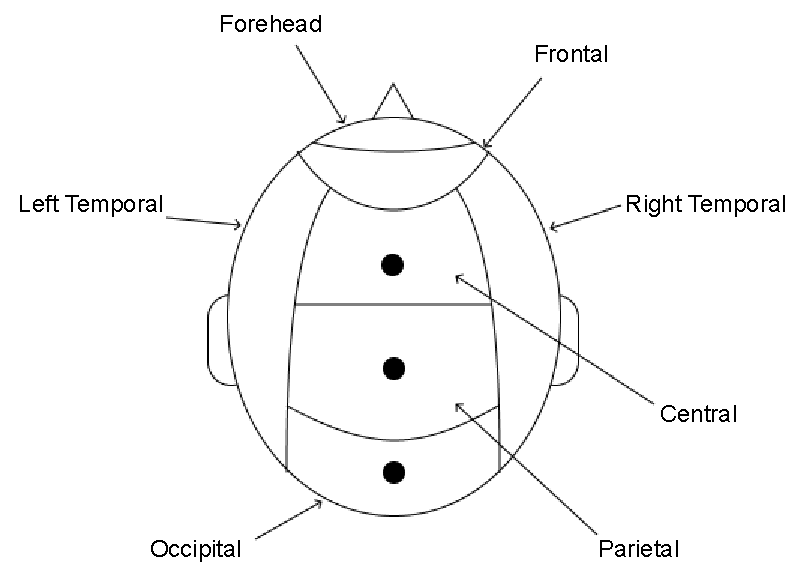
\includegraphics[width=0.60\textwidth]{images/head-regions.pdf}
    \caption{Diagram shows the different regions of the head, as well as the placement of the tactors for our described system.}
    \label{fig:head-regions}
\end{figure}

\section{Evaluation}

Graphs are always good. I recommend getting to grips with Matlab, R or
gnuplot rather than exporting horribly Excel bitmapped graphs.


\begin{quotation}
 The Assyrian came down like the wolf on the fold,
 And his cohorts were gleaming in purple and gold;
 And the sheen of their spears was like stars on the sea,
 When the blue wave rolls nightly on deep Galilee.

 Like the leaves of the forest when Summer is green,
 That host with their banners at sunset were seen:
 Like the leaves of the forest when Autumn hath blown,
 That host on the morrow lay withered and strown.
\end{quotation}

\begin{table}
\begin{tabular}{l||c||p{2cm}}
\emph{Operating System} & \emph{Version} & \emph{Verdict} \\ \hline \hline
Ubuntu & 12.04 & Everyone's favourite Linux, unless you grew up with
RedHat \\ \hline
Slackware & xxx & Pseudo-hacker's Linux, how often do you recompile
your kernel? \\ \hline
Mac OS & 10.7 & For people with more money than sense \\ \hline
\end{tabular}
\caption{\label{tab-eg}Single column table of figures}
\end{table}

\begin{figure*}
\begin{center}

\includegraphics[scale=0.3]{alice.pdf}
\end{center}
\caption{\label{fig-eg}An example figure stretching over two columns}
\end{figure*}

\section{Conclusions}

The standard Lorem Ipsum passage, used since the 1500s

``Lorem ipsum dolor sit amet, consectetur adipisicing elit, sed do eiusmod tempor incididunt ut labore et dolore magna aliqua. Ut enim ad minim veniam, quis nostrud exercitation ullamco laboris nisi ut aliquip ex ea commodo consequat. Duis aute irure dolor in reprehenderit in voluptate velit esse cillum dolore eu fugiat nulla pariatur. Excepteur sint occaecat cupidatat non proident, sunt in culpa qui officia deserunt mollit anim id est laborum.''
\vskip8pt \noindent
{\bf Acknowledgments.}
This is optional; it is a location for you to thank people, most probably your family and your supervisor.

\bibliographystyle{abbrv}
\bibliography{example}


\end{document}
